\subsection{Pisa/IIT SoftHand}
\label{sec:softhand}

The Pisa/IIT SoftHand is a 5-finger hand that introduces an implementation of the adaptive synergy transmission~\cite{Catalano2014Adaptive}. Fig~\ref{fig:soft_hand}.

\begin{figure}[b]
\centering
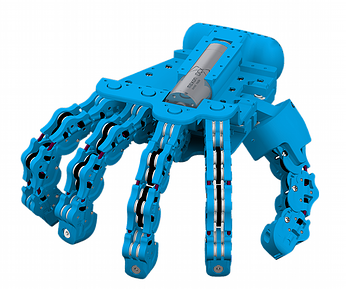
\includegraphics[width=0.4\textwidth]{soft_hand.png}
\caption{The Pisa/IIT SoftHand, 1 motor and 19 dof.}
\label{fig:soft_hand}
\end{figure}

\subsubsection{Hardware interface}

The real hardware interface is implemented using the API provided by qbrobotics$^{\copyright}$~\cite{qbrobotics_software}, using position commands. 

The simulated hardware interface is special. 

The interface is loaded into Gazebo as a plug-in that has access to the simulation, useful to read the full hand state as well as contacts, and receives commands from the controller in position. To simulate the SoftHand behavior the four elements described below are used within the interface implementation.

\paragraph{Joint description} The knuckle joint for all fingers is a regular revolute joint, so they are specified as such using common URDF tags~\ref{webros}. The inter-phalangeal joints, however, are based compliant rolling-contact joints, which are not among the library of joint types in any of the simulation environments available today, as far as the authors know. Thus, it requires a special treatment to emulate the kinematic motion resulting from rolling. To this end, each inter-phalangeal joint is the combination of two revolute joints having the same angle, that is, coupled with the same ratio to the reduced synergy actuator. For more details on this, see the preliminary work of modeling the Pisa/IIT SoftHand in ADAMS (in Italian, but the subject can be followed readily)~\cite{Piazza2013Studio}, available at~\href{./attachedPapers/CristinaPiazzaReport.pdf}{this link}.

\paragraph{Transmission interface} This part contains the mapping between the actuator (one motor) and joints (19 revolute joints and 19 mimic joints) in position and effort domains. That is, according to~\cite{Catalano2014Adaptive}, actuating the adaptive synergistic hand by direct control of the reduced synergy vector $\sigma^{1}$, leads to the system
\begin{equation}
\left[ \begin{array}{cc} -E & R^{T} \\ R & 0 \end{array} \right] \left[ \begin{array}{c} q \\ R  \end{array} \right] = \left[ \begin{array}{c} J^{T}f_{c} \\ \sigma^{1}  \end{array} \right],
\end{equation}
where $E$ is the joint space stiffness matrix, $R$ is the transmission ratio matrix, $q$ the reference position of the springs in the phalanges, $J$ is the grasp Jacobian and $f_c$ is the wrench associated with the contact forces. The solution to this system was implemented for the different mappings between actuator and joints.

\paragraph{Contact wrenches $f_c$} An out-of-the-box Gazebo plug-in is available that is loaded per each body, i.e. each phalanx, that provides all contact point and wrenches, as well as the resultant wrench at the body reference frame. The later is particularly useful for the next element.

\paragraph{Grasp Jacobian $J$} A kinematic library is used to obtained all Jacobian's that relate all phalanges to the different finger sub-chains. That is, for one finger with 4 joints, 4 Jacobian's are computed at the current hand joint state, namely, the consideration of 4, 3, 2, and 1 joints, respectively. Since the total contact wrench per phalanx is already expressed in the phalanx reference frame, the Jacobian's are obtained using that as the reference frame, and the palm as the base frame. 

To illustrate the implementation, Fig.~\ref{fig:soft_hand_gazebo} shows the hand prior to closing and after closing, with an obstacle in the middle. Recall that the only actuation is the synergy motor, and the rest of joints are commanded through the implementation of the adaptive synergy transmission as described above.

\begin{figure}
\centering
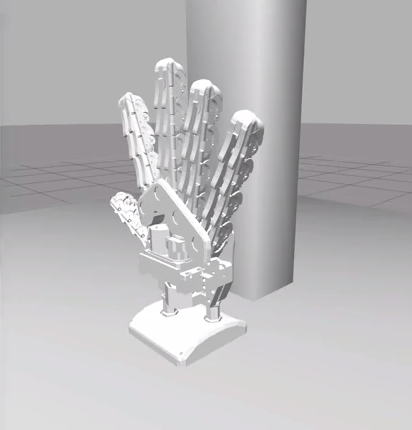
\includegraphics[width=0.45\textwidth]{open.png}
\hspace{1pt}
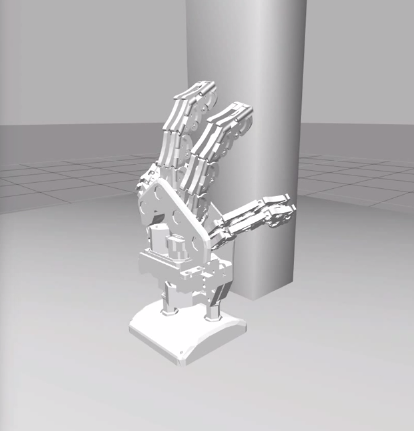
\includegraphics[width=0.45\textwidth]{close.png}
\caption{The Pisa/IIT SoftHand simulated in Gazebo at full open (left) and close (right) commanded configurations.}
\label{fig:soft_hand_gazebo}
\end{figure}

\subsubsection{Joint state estimation}

At this point, there are two on going works regarding this issue that we expect to converge in a sensor fusion approach during the time remaining on the project. The first one is presented in DR 3.1, where an IMU-based glove provides an accurate estimate of the joint angles. The second approach is a simulator-in-the-loop extended Kalman filter, where the simulation play the role of the system model to give the estimated joint values, and motor position (via a position encoder) and effort (estimated from the current measurement) are used as measurements to update the filter via the adaptive synergy transmission equations implemented in the transmission interface as described above. This work is being submitted to IROS 2015, for more details see the attached at~\href{}{this link}.